Um Web-Components besser verstehen zu können, wird in diesem Kapitel zu Beginn eine kurze Übersicht über die Entstehung von diversen Web-Bibliotheken gezeigt. Sämtliche Bibliotheken dienen der benutzerdefinierten Erstellung von Komponenten, oder stellen selbst eine Reihe von benutzbaren Komponenten bereit. Ein nennbare Schwäche hierbei ist, das sämtliche Komponenten nicht Interoperabel sind, ohne die Basisbibliotheken zu inkludieren.

Die aufgelisteten Bibliotheken wurden an Hand der Popularität auf Github ausgewählt. Neben den genannten Bibliotheken gibt es jedoch eine Vielzahl anderer Projekte, die für einen kurzen und minimalen Überblick nicht genannt werden.

\begin{description}
\item[2005:] Veröffentlichung von Dojo Toolkit\footnote{Mehr Information zu Dojo Toolkit auf \href{http://dojotoolkit.org/}{http://dojotoolkit.org/}} mit der innovativen Idee von Widgets. Mit ein paar Zeilen Code konnten Entwickler komplexe Elemente, wie beispielsweise einen Graph oder eine Dialog-Box in ihrer Website hinzufügen \citereset \autocite[siehe][]{Dojo.2005}.
\item[2006:] jQuery\footnote{Mehr Information zu jQuery auf \href{http://jquery.com/}{http://jquery.com/}} stellt Entwicklern die Funktion zur Verfügung Plugins zu entwickeln, die später wiederverwendet werden können \citereset \autocite[siehe][]{jQuery}.
\item[2008:] Veröffentlichung von jQuery-UI\footnote{Mehr Information zu jQuery UI auf \href{http://jqueryui.com/}{http://jqueryui.com/}}, was vordefinierte Widgets und Effekte mit sich bringt \citereset \autocite[siehe][]{jQueryUI}.
\item[2009:] Erstveröffentlichung von AngularJS\footnote{Mehr Information zu AngularJS auf \href{http://angularjs.org/}{http://angularjs.org/}}, ein Framework mit Direktiven \citereset \autocite[siehe][]{AngularJS}.
\item[2011:] Erstveröffentlichung von React\footnote{Mehr Information zu Facebook React auf \href{http://facebook.github.io/react/}{http://facebook.github.io/react/}}. Diese Bibliothek gibt den Entwicklern die Fähigkeit, das User Interface ihrer Website zu bauen, ohne dabei auf andere Frameworks, die auf der Seite benutzt werden, achten zu müssen \citereset \autocite[siehe][]{Facebook}.
\item[2013:] Veröffentlichung der Spezifikation von Web-Components \citereset \autocite[siehe][]{CooneyGlazkov.2013}
\end{description}

Web-Components ist ein Komponentenmodell, das 2013 in einem Working-Draft des W3C veröffentlicht wurde. Es besteht aus fünf Teilen:
\begin{description}
\item[HTML Templates] beinhalten Markup, das vorerst inaktiv ist, aber bei späterer Verwendung aktiviert werden kann. Auch kann das definierte Markup in einem Template vervielfältigt werden und dient somit der Wiederverwendbarkeit (ausführliche Erklärung siehe Kapitel \ref{sec:3_WC_Templates} auf Seite \pageref{sec:3_WC_Templates}).
\item[Decorators] verwenden CSS-Selektoren basierend auf den Templates, um visuelle beziehungsweise verhaltensbezogene Änderungen am Dokument vorzunehmen (ausführliche Erklärung siehe Kapitel \ref{sec:3_WC_Decorators} auf Seite \pageref{sec:3_WC_Decorators}).
\item[Custom Elements] können neue Elemente definieren, oder bereits bestehende Elemente erweitern (ausführliche Erklärung siehe Kapitel \ref{sec:3_WC_Elements} auf Seite \pageref{sec:3_WC_Elements}).
\item[Shadow DOM] erlaubt es eine DOM-Unterstruktur vollständig zu kapseln. Sämtliche Elemente in dieser Unterstruktur sind von außen nicht erreichbar. Somit werden zuverlässigere Benutzerschnittstellen der Elemente garantiert, da keine Interferenzen in den Unterstrukturen entstehen können (ausführliche Erklärung siehe Kapitel \ref{sec:3_WC_Shadow_DOM} auf Seite \pageref{sec:3_WC_Shadow_DOM}).
\item[HTML Imports] definieren, wie Templates, Decorators und Custom Elements verpackt und als eine Ressource geladen werden können. (ausführliche Erklärung siehe Kapitel \ref{sec:3_WC_Imports} auf Seite \pageref{sec:3_WC_Imports}).
\end{description}

Beispielsweise könnte ein HTML-Element von einer einfachen Überschrift mit fest definiertem Aussehen, über einen Videoplayer, bis hin zu einer kompletten Applikation, darstellen. Vieles, was derzeit über Javascript-Bibliotheken abgewickelt wird, könnte künftig in Form einzelner Webkomponenten umgesetzt werden. Das verringert Abhängigkeiten und sorgt für mehr Flexibilität.

Obwohl \glqq Web-Components\grqq\ für viele Entwicklerinnen und Entwickler noch kein Begriff ist, wird es bereits von diversen Browsern verwendet. Beispiele hierfür sind der \glqq Datepicker\grqq , oder das \lstinline|<video>|-Element. Abbildung \ref{fig:3_Datepicker_Visuals} auf Seite \pageref{fig:3_Datepicker_Visuals} zeigt die Datepicker-Komponente und Abbildung \ref{fig:3_Datepicker_Source} auf Seite \pageref{fig:3_Datepicker_Source} zeigt den dazugehörigen Quellcode. An Hand dieses Codes ist zu sehen, dass sämtliche Kontrollbuttons des Datepickers \glqq versteckt\grqq sind, sprich im Shadow-DOM liegen.


\begin{figure}[h]
\centering
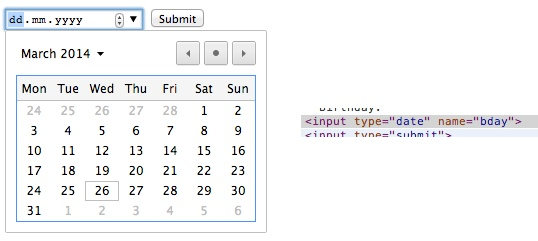
\includegraphics[height=5.0cm]{images/datepicker.jpg}
\caption[
Beispiel von Web-Components im Browser an Hand eines Datepickers, Urldate: 04.2014
\newline
\small\texttt{\url{https://s3.amazonaws.com/infinum.web.production/repository\_items/files/000/000/238/original/datepicker.jpg}}
]{Beispiel von Web-Components im Browser an Hand eines Datepickers}
\label{fig:3_Datepicker_Visuals}
\end{figure}

\begin{figure}[h]
\centering
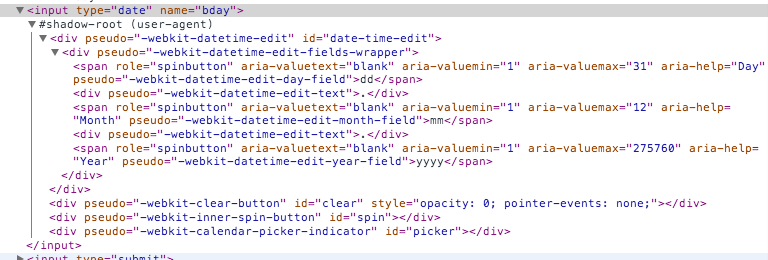
\includegraphics[height=5.0cm]{images/datepicker_shadow_dom.jpg}
\caption[
Beispiel von Web-Components im Browser an Hand eines Datepickers, Urldate: 04.2014
\newline
\small\texttt{\url{https://s3.amazonaws.com/infinum.web.production/repository\_items/files/000/000/236/original/datepicker\_shadow\_dom.jpg}}
]{Beispiel von Web-Components im Browser an Hand eines Datepickers}
\label{fig:3_Datepicker_Source}
\end{figure}

\textbf{Warum Web-Components?}

Javascript Widgets und Plugins sind fragmentiert, weil sie auf diversen unterschiedlichen Bibliotheken und Frameworks basieren, die oftmals nicht interoperabel sind. Web-Components versuchen einen Standard in Widgets und Plugins zu bringen. Das Problem der nicht miteinander funktionierenden Plugins wird bei Web-Components mit Kapselung gelöst. Durch die Lösung dieses Problems ist die Wiederverwendbarkeit von Komponenten garantiert, da es sämtliche Interferenzen zwischen Plugins löst. Web-Components können des Weiteren viel mehr als nur UI-Komponenten sein.

\textbf{Unterstützung von Web-Components}

Zur Zeit ist die Hauptproblematik von Web-Components die mangelhafte Browser-Unterstützung. Kein einziger Browser unterstützt diesen Standard zu 100\%. Es gibt bereits mehrere Möglichkeiten beziehungsweise Polyfills\footnote{Ein Polyfill ist ein Browser-Fallback, um Funktionen, die in modernen Browsern verfügbar sind, auch in alten Browsern verfügbar zu machen.}, um dennoch Web-Components nutzen zu können. Beispiele hierfür sind:
\begin{itemize}
\item Polyfill-Webcomponents\footnote{Mehr Information zu Polyfill-Webcomponents unter \href{http://github.com/timoxley/polyfill-webcomponents}{http://github.com/timoxley/polyfill-webcomponents}}
\item Polymer-Project\footnote{Mehr Information zu Polymer unter \href{http://www.polymer-project.org/}{http://www.polymer-project.org/}}
\item X-tags\footnote{Mehr Information zu X-tags unter \href{http://x-tags.org/}{http://x-tags.org/}}
\end{itemize}

Dadurch, dass der Spezifikation von Web-Components Kapselung vorschreibt, sind sämtliche Polyfills interkompatibel.

Diese Arbeit beschränkt sich hauptsächlich auf die Entwicklung von Web-Components mit Hilfe des Standards beziehungsweise der Polyfill-Bibliothek Polymer.

Durch die Benutzung von dem Polyfill namens Polymer funktionieren Web-Component in allen \glqq Evergreen\grqq -Browser\footnote{Ein \glqq Evergreen\grqq -Browser ist ein Web-Browser, der sich automatisch beim Start updatet.} und Internet-Explorer 10 und neuer. Folglich funktionieren sie auch auf mobilen Endgeräten, wo iOS6+, Chrome Mobile, Firefox Mobile, oder Android 4.4 oder höher vorhanden ist.